\chapter{Stratégie}
\label{cp:strategie}

La stratégie utilisée pour terminer le jeu est construite autour de l'algorithme A* (\autoref{sec:a-star}).
\newline
On commence par récupérer la liste des bonus par ordre croissant de distance, et on essaie, en utilisant A*, de trouver un chemin pour atteindre le bonus le plus proche.
\newline
Si on trouve un chemin vers un des bonus, le runner le prendra : A* a une priorité sur toutes les autres décisions.
\newline
Si l'algorithme ne trouve aucun chemin vers aucun bonus (au plus il y a d'ennemis, au plus ça arrive), le runner utilise des fonctions de mouvements dites "spéciales" pour se déplacer.
\newline\newline
Ceci veut dire que A* doit prendre en compte les ennemis, mais il y a plusieurs avantages à utiliser cette stratégie :

\begin{enumerate}
    \item On fait une confiance totale à A* : s'il sait qu'un ennemi n'est pas dangereux, il n'y a pas besoin de faire de mouvements pour l'éviter.
    \item On ne fait pas de mouvements inutiles : si A* trouve un chemin, on peut prouver que c'est le chemin le plus court.
    \item Si A* ne trouve pas de chemin, on peut être sûr qu'il n'y en a pas, et on peut donc se permettre de faire des mouvements "spéciaux".
\end{enumerate}
Néanmoins, il y a un inconvénient : on ne peut pas prédire l'évolution de la position des ennemis, les choix de A* se basent sur la situation à l'instant $t$.
C'est pour cela qu'on l'appelle à chaque tour, pour prendre en compte les nouvelles positions des ennemis.
\newline\newline
Heureusement, l'imprécision de la position des ennemis augmente avec la distance, et leur dangerosité diminue.
L'algorithme peut être à peu près sûr de la position des ennemis proches (les ennemis dangereux), et donc de les éviter.

\newpage

\begin{figure}[!htpb]
    \centering
    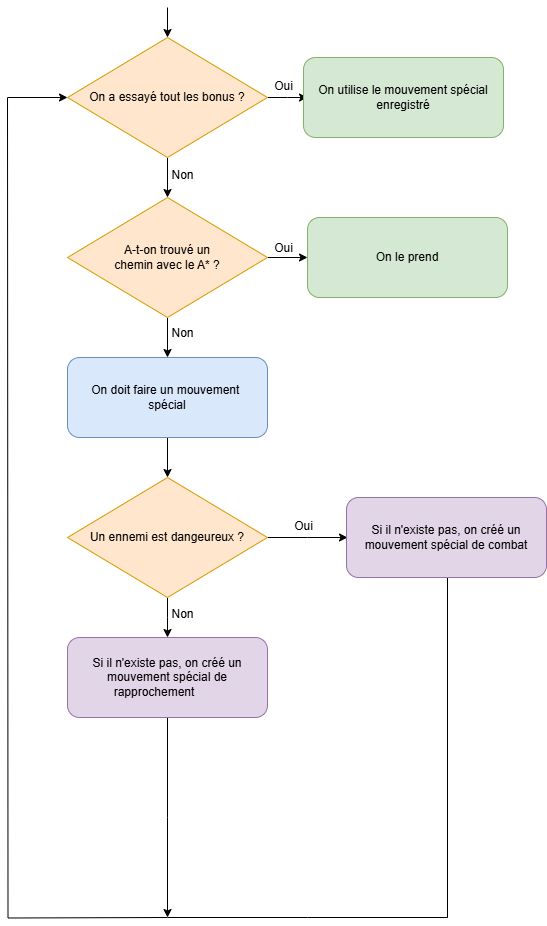
\includegraphics[width=0.75\linewidth]{Figures/diagramme2.png}
    \caption[Logigramme de la stratégie.]{Logigramme de la stratégie.}
    \label{fig:logigramme}
\end{figure}

\section{Mouvements spéciaux}

Les mouvements spéciaux sont les mouvements effectués quand A* ne trouve aucun chemin, ils tentent, sans garantie de succès, d'améliorer la situation pour que A* puisse trouver un chemin lors d'un prochain tour.
\newline
Ils sont, contrairement à A*, beaucoup plus spécifiques.

\subsection{Mouvement de combat}

Comme vu dans le logigramme (\autoref{fig:logigramme}), un mouvement de combat est enregistré si A* ne trouve aucun chemin, qu'un ennemi est considéré comme dangereux (\autoref{sec:ennemi-dangereux}) et qu'il n'existe pas déjà un mouvement de combat.
Alors, on va utiliser une suite de conditions (\autoref{sec:move-to-combat}) pour déterminer l'action à réaliser (se déplacer, poser une bombe, attendre).

\subsection{Mouvement de rapprochement}

Si A* ne trouve aucun chemin et qu'aucun ennemi n'est considéré comme dangereux, c'est qu'un ou plusieurs ennemis bloquent le chemin.
On va alors essayer de se rapprocher du bonus, jusqu'à ce que : 
\begin{itemize}
    \item A* trouve un chemin.
    \item On se rapproche assez d'un ennemi pour qu'il soit considéré comme dangereux.
\end{itemize}

\subsection{Remarques}

Il faut faire attention à bien conserver le premier mouvement de combat (et de rapprochement), car on va itérer sur tous les bonus, mais on souhaite se rapprocher du plus proche (le premier). 